\documentclass{article}
\usepackage{amsmath}
\usepackage{amssymb}
\usepackage{amsthm}
\usepackage{amsfonts}
\usepackage[margin=2cm]{geometry}
\usepackage{graphicx}
\usepackage{color}
\usepackage[all]{xy}
\newtheorem*{lem}{Lemma}

\title{Solution for Exercise sheet 7}
\author{Yikai Teng, You Zhou}
\date{Exercise session: Thu. 8-10}
\begin{document}
\maketitle
\paragraph{Exercise 7.1}Fix some $x\in X.$ For every open neighborhood $O$ of $f(x),$ since $f(x)\in W(\{x\},O)$ and $f_n\stackrel{c.o.}\rightarrow f,$ there exists some $N>0$ such that $n>N$ implies that $f_n\in W(\{x\},O),$ i.e. $f_n(x)\in O.$ So $f_n(x)$ converges to $f(x).$

For a counterexample, consider $X=[0,1]$ and $Z=\mathbb{R}$ with the usual metric. Then under the supreme metric $Z^X$ is a metric space and the compact open topology on $Z^X$ coincides with the metric topology induced by the supreme metric. Hence in this case convergence in compact open topology of is the same as uniform convergence. There are many sequences of functions from $[0,1]$ to $\mathbb{R}$ that converge pointwise but not uniformly, for example $\{f_n(x)=nxe^{-nx}\}$ satisfies $\lim_{n\rightarrow\infty}f_n(x)=0$ for every fixed $x$ but $f_n(\frac{1}{n})=e^{-1},$ which shows that $\{f_n\}$ cannot converge uniformly.

\paragraph{Exercise 7.3}
We first see what each map does separately and then combine them together. First consider $\pi_0(\Phi).$ For some $f\in E,$ let $[f]$ denote the path component represented by $f$ in $\pi_0(E).$ Then by definition
\[\pi_0(\Phi)([f])=[\Phi(f)]=[(f\circ i,f\circ j)]\in\pi_0(\Omega X\times\Omega X),\]
where $i$ and $j$ are as in exercise 6.3. By our construction in exercise 6.3, its inverse can be described as
\[\pi_0(\Phi)^{-1}([(f,g)]):=[\alpha(f,g)]\in\pi_0(E),\]
which is illustrated in the figure \ref{7.3_1} below.
\begin{figure}[ht]
  \centering
  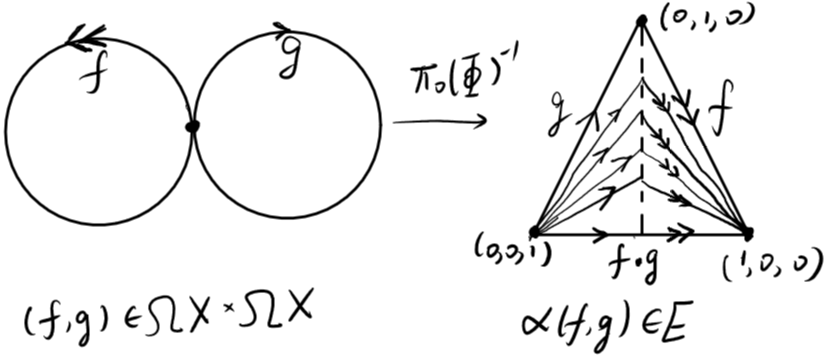
\includegraphics[width=8cm]{7.3_1.png}
  \caption{Illustration of $\pi_0(\Phi)^{-1}$}\label{7.3_1}
\end{figure}

Then consider $\pi_0(\sigma^*).$ For some $[f]\in\pi_0(E),$ by definition $\pi_0(\sigma^*)([f])=[f\circ\sigma_*].$

Now combine them together and see what $[(f,g)]\in\pi_0(\Omega X\times\Omega X)$ becomes after this composite. First $\pi_0(\Phi)^{-1}([(f,g)]):=[\alpha(f,g)],$ as shown in figure \ref{7.3_1} above. Then $\pi_0(\Phi)\circ\pi_0(\sigma^*)([\alpha(f,g)])=[(\alpha(f,g)\circ\sigma_*\circ i,\alpha(f,g)\circ\sigma_*\circ j)].$ The representative has six possibilities, i.e.
\begin{equation}\label{1}
  (\alpha(f,g)\circ\sigma_*\circ i,\alpha(f,g)\circ\sigma_*\circ j)=
\begin{cases}
  (f,g), & \mbox{if } \sigma=\text{id} \\
  (f^{-1},f\cdot g), & \mbox{if } \sigma=(01) \\
  (g^{-1},f^{-1}), & \mbox{if } \sigma=(02) \\
  (f\cdot g,g^{-1}), & \mbox{if } \sigma=(12) \\
  (g,(f\cdot g)^{-1}), & \mbox{if } \sigma=(012) \\
  ((f\cdot g)^{-1},f), & \mbox{if } \sigma=(021).
\end{cases}
\end{equation}
where $f\cdot g(t):=\alpha(f,g)(t,0,1-t)$ and $f^{-1}(i(t))$ is given by $f(i(1-t)).$ As an example I explain the second one in more detail. Here $\sigma=(01)$ and
\begin{gather*}
  \alpha(f,g)\circ\sigma_*\circ i(t)=\alpha(f,g)\circ\sigma_*(t,1-t,0)=\alpha(f,g)(1-t,t,0)=f\circ i(1-t),\\
  \alpha(f,g)\circ\sigma_*\circ j(t)=\alpha(f,g)\circ\sigma_*(0,t,1-t)=\alpha(f,g)(t,0,1-t)=f\cdot g(t).
\end{gather*}
In general we don't know the relation between $f,g,f\cdot g$ and their inverses as elements of $\pi_1(X),$ so \eqref{1} gives explicitly the operation of the composite.
\end{document} 